%%%%%%%%%%%%%%%%%%%%%%%%%%%%%%%%%%%%%%%%%%%%%%%%%%%%%%%%%%%%
%%% ELIFE ARTICLE TEMPLATE
%%%%%%%%%%%%%%%%%%%%%%%%%%%%%%%%%%%%%%%%%%%%%%%%%%%%%%%%%%%%
%%% PREAMBLE 
\documentclass[9pt,lineno]{elife}
% Use the onehalfspacing option for 1.5 line spacing
% Use the doublespacing option for 2.0 line spacing
% Please note that these options may affect formatting.
% Additionally, the use of the \newcommand function should be limited.

\usepackage{lipsum} % Required to insert dummy text
\usepackage[version=4]{mhchem}
\usepackage{siunitx}
\DeclareSIUnit\Molar{M}

%%%%%%%%%%%%%%%%%%%%%%%%%%%%%%%%%%%%%%%%%%%%%%%%%%%%%%%%%%%%
%%% ARTICLE SETUP
%%%%%%%%%%%%%%%%%%%%%%%%%%%%%%%%%%%%%%%%%%%%%%%%%%%%%%%%%%%%
\title{Sex-Specific Evolution of the Meiotic Recombination Rate}

\author[1*]{April L. Peterson}
\author[1,2\authfn{1}\authfn{3}]{Bret Payseur}
\affil[1]{University of Wisconsin-Madison}


\corr{email1@example.com}{FMS}
\corr{email2@example.com}{FS}

\contrib[\authfn{1}]{These authors contributed equally to this work}
\contrib[\authfn{2}]{These authors also contributed equally to this work}

\presentadd[\authfn{3}]{Department, Institute, Country}
\presentadd[\authfn{4}]{Department, Institute, Country}
% \presentadd[\authfn{5}]{eLife Sciences editorial Office, eLife Sciences, Cambridge, United Kingdom}

%%%%%%%%%%%%%%%%%%%%%%%%%%%%%%%%%%%%%%%%%%%%%%%%%%%%%%%%%%%%
%%% ARTICLE START
%%%%%%%%%%%%%%%%%%%%%%%%%%%%%%%%%%%%%%%%%%%%%%%%%%%%%%%%%%%%

\begin{document}

\maketitle

\begin{abstract}
Although meiotic recombination is required for successful gametogenesis in most species that reproduce sexually, the rate of crossing over varies among individuals. Differences in recombination rate between females and males are perhaps the most striking form of this variation. Existing data fail to directly address the extent to which recombination experiences similar evolutionary pressures. To fill this gap, we measured meiotic recombination in both sexes for a panel of house mouse cross three subspecies. Using inbred strains and single cell immunohistochemistry allowed us to place sex-specific observations within the same genetic background and meiotic context. Our results indicate highly discordant evolutionary patterns in the two sexes. Whereas male recombination rates show evidence of rapid evolution over short evolutionary timescales, female recombination rates measured in the same strains are mostly static. These results strongly indicate that house mouse has two genome wide recombination rates which display distinct evolutionary trajectories. 
\end{abstract}


\section{Introduction (Level 1 heading)}

Thanks for using Overleaf to write your article. Your introduction goes here! Some examples of commonly used commands and features are listed below, to help you get started.

Here's a second paragraph to test paragraph indents. \lipsum[1]

\section{Results (Level 1 heading)}


\subsection{Genome-wide recombination rate evolves differently in females and males} 

We used counts of MLH1 foci per cell to estimate genome-wide recombination rates in `r length(unique(  (main.table  %>% filter(species == "M.musculus") )$strain) )` wild-derived inbred strains sampled from three subspecies of house mice (*M. m. domesticus*, _M. m. musculus_ and _M. m. molossinus_ ) and three additional species of Mus (*M. spretus*, _M. spicilegus_ , and *M. caroli*). Mean MLH1 focus counts for `r sum(main.table$Nmice)` mice were quantified from an average of `r mean( (Mouse.Table_HQ %>% filter(sex == "male") )$Ncells, na.rm = T)` spermatocytes per male (for a total of `r formatC( sum( (Mouse.Table_HQ %>% filter(sex == "male") )$Ncells, na.rm = T), format="d", big.mark=",")` spermatocytes) and `r mean( (Mouse.Table_HQ %>% filter(sex == "female") )$Ncells, na.rm = T)` oocytes per female (for a total of `r formatC(sum( (main.table %>% filter(species == "M.musculus") %>% filter(sex == "female"))$Ncells), format="d", big.mark=",")` oocytes).

\subsection{Synaptonemal complexes are longer in females}


\subsection{Females and males differ in crossover positions and crossover interference}


\subsection{Evolution of genome-wide recombination rate is dispersed across bivalents, associated with double-strand break number, and connected to crossover interference}


\section{Discussion}

By comparing recombination rates in females and males from the same diverse set of genetic backgrounds, we isolated sex as a primary factor in the evolution of this fundamental meiotic trait. Recombination rate differences are more pronounced in males than females. Because inter-strain divergence times are identical for the two sexes, this observation demonstrates that the genome-wide recombination rate evolves faster in males, at least in house mice. More generally, recombination rate divergence is decoupled in females and males. These disparities are remarkable given that recombination rates for the two sexes were measured in identical genomic backgrounds (other than the presence/absence of the Y chromosome). Our results provide the strongest evidence yet that the genome-wide recombination rate follows distinct evolutionary trajectories in males and females.

At the genetic level, the sex-specific evolution we documented indicates that some mutations responsible for divergence in recombination rate have dissimilar phenotypic effects in females and males. A subset of the genetic variants associated with genome-wide recombination rate within populations of humans \citep{Kong2004, Kong2008, Kong2014, halldorsson2019}, Soay sheep \citep{johnston2016_soay}, and cattle  \citep{ma2015_cattle, Shen2018_cattle} appear to show sex-specific properties, including opposite effects in females and males. Furthermore, inter-sexual correlations for recombination rate are weak in humans \citep{fledel2011} and Soay sheep \citep{johnston2016_soay}. Crosses between the strains we surveyed could be used to identify and characterize the genetic variants responsible for recombination rate evolution in house mice \citep{dumont2011, Wang2017island, wang2019_SC}. These variants could differentially affect females and males at any step in the recombination pathway. Although our DMC1 profiling was limited to males from a small number of strains (for practical reasons), our findings suggest that mutations that determine the number of double-strand breaks contribute to sex-specific evolution in the recombination rate. A study of two classical inbred strains and one wild-derived inbred strain of house mice also found a positive association between crossover number and double-strand break number in males \citep{baier2014}.

Another implication of our results is that the connection between recombination rate and fitness differs between males and females. Little is known about whether and how natural selection shapes recombination rate in nature \citep{DapperPayseur2017, Ritz2017}.  \cite{samuk2020} recently used a quantitative genetic test to conclude that an 8 percent difference in genome-wide recombination rate between females from two populations of *Drosophila pseudoobscura* was caused by natural selection. Applying similar strategies to species in which both sexes recombine, including house mice, would be a logical next step to understanding the sex-specific evolution of recombination rate. 

Population genetic models have been built to explain sexual dimorphism in the number and placement of crossovers, which is a common phenomenon \citep{brandvain2012scrambling, sardell_sex_2020}. Modifier models predicted that lower recombination rates in males will result from haploid selection \citep{lenormand2003} or sexually antagonistic selection on coding and cis-regulatory regions of genes \citep{sardell_sex_2020}. Another modifier model showed that meiotic drive could stimulate female-specific evolution of the recombination rate \citep{brandvain2012scrambling}. Although these models fit the conserved pattern of sex differences in crossover positions, they do not readily explain our observations of sex-specific evolution in the genome-wide recombination rate. In particular, the alternation across strains in which sex has more crossovers is unexpected.

We propose an alternative interpretation of our findings based on the cell biology of gametogenesis. During meiosis, achieving a stable chromosome structure requires the attachment of kinetochores to opposite poles of the cell and at least one crossover to create tension across the sister chromosome cohesion distal to chiasmata \citep{LaneKauppi2019, vanVeen2003}. The spindle assembly checkpoint (SAC) prevents aneuploidy by ensuring that all bivalents are correctly attached to the microtubule spindle (“bi-oriented”) before starting the metaphase-to-anaphase transition via the release of the sister cohesion holding homologs together \citep{LaneKauppi2019}. Hence, selection seems likely to favor mutations that optimize the process of bi-orientation and chromosome separation, thereby prohibiting the SAC from delaying the cell cycle or triggering apoptosis. Multiple lines of evidence indicate that the SAC is more effective in spermatogenesis than in oogenesis [@LaneKauppi2019], perhaps due to the presence of the centrosome spindle \citep{So2019} and larger cell volume \citep{kyogoku2017} in oocytes. The higher stringency of the SAC during spermatogenesis suggests that selection will be better at removing mutations that interfere with bi-orientation in males than in females. Therefore, faster male evolution of the genome-wide recombination rate could be driven by the more stringent SAC acting on chromosome structures at the metaphase I alignment.


Our SAC model is consistent with other features of our data. We showed that widespread sex differences in broad-scale crossover positioning \citep{sardell_sex_2020} apply across house mice, even in lineages where the direction of heterochiasmy is reversed. The number and placement of crossovers affects the area of sister chromosome cohesion distal to crossovers which needs to be released for the first reductional chromosome segregation \citep{vanVeen2003, LaneKauppi2019, subramanian2014, dumontDesai2012}. Faster spermatogenesis may select for synchronization of the separation across all homologs within the cell (**Kudo** ), whereas in oogenesis, the slower cell cycle and multiple arrest stages may require chromosome structures with greater stability on the MI spindle, especially for those organisms that undergo dictyate arrest \citep{Lee2019}.

We propose that the SAC model also can explain the correlated evolution of stronger crossover interference and higher genome-wide recombination rate in male house mice. Our results show that crossovers are spaced further apart in strains enriched for double-crossover bivalents when SC length is taken into account and chromosome size effects are minimized. Assuming chromatin compaction between (prophase) pachytene and metaphase is uniform along bivalents, this increased spacing is expected to expand the area for sister cohesion to connect homologs and may improve the fidelity of chromosomal segregation. While the SAC model postulates direct fitness effects of interference, a modifier model predicted that indirect selection on recombination rate – via its modulation of offspring genotypes – can strengthen interference as well \citep{goldstein1993}.

Regardless of the underlying mechanism, our results provide a rare demonstration that crossover interference can diverge over short evolutionary timescales. The notion that stronger interference can co-evolve with higher genome-wide recombination rate is supported by differences between breeds of cattle \citep{ma2015_cattle} and differences between populations of white-footed mice \citep{peterson2019}. In contrast, mammalian species with stronger interference tend to exhibit lower genome-wide recombination rates \citep{segura2013, @ottoPaysuer2019}. Collectively, these patterns suggest that inferences about the evolutionary dynamics of interference depend on the timescale under consideration.

Our findings further reveal that evolution of the genome-wide recombination rate does not require major changes in the degree of chromatin compaction. Female house mice consistently show longer SCs, even in strains with more recombination in males. Studies in mice \citep{lynn2002, petkov2007} and humans \citep{gruhn2013, tease2004} suggest that chromosomal axes are longer (and DNA loops are shorter) in females than males. Some authors have suggested that conserved sex differences in crossover positioning (more uniform placement in females) and interference strength (stronger interference in males) could be due to looser chromatin packing of the meiotic chromosome structure in females \citep{haenel2018; @petkov2007}. A cellular model designed to explain interference attributes sexual dimorphism in chromatin structure to greater cell volumes and oscillatory movements of telomeres and kinetochores in oocytes \citep{@hulten2011_COM}. More recent work connects the sparser recombination landscape to sex differences in the crossover repair pathway \citep{wang2017inefficient}.

Our conclusions are accompanied by several caveats. First, MLH1 foci only identify interfering crossovers \citep{holloway2008mus81}. Although most crossovers belong to this class **(REF)**, our approach likely underestimated genome-wide recombination rates. Evolution of the number of non-interfering crossovers is a topic worth examining. A second limitation is that our investigation of crossover locations was confined to the relatively low resolution possible with immunofluorescent cytology. Positioning crossovers with higher resolution could reveal additional evolutionary patterns. Finally, the panel of inbred lines we surveyed may not be representative of recombination rate variation within and between subspecies of house mice. We considered most available wild-derived inbred lines, but house mice have a broad geographic distribution. Nevertheless, we expect our primary conclusion that recombination rate evolves in a sex-specific manner to be robust to geographic sampling because differences between females and males exist for the same set of inbred strains.

While the causes of sex differences in recombination remain mysterious \citep{lenormand2016}, our conclusions have implications for a wide range of recombination research. For biologists uncovering the cellular and molecular determinants of recombination, our results suggest that mechanistic differences between the sexes could vary by genetic background. For researchers charting the evolutionary trajectory of recombination, our findings indicate that sex-specific comparisons are crucial. For theoreticians building evolutionary models of recombination, different fitness regimes and genetic architectures in females and males should be considered. Elevating sex as a primary determinant of recombination would be a promising step toward integrating knowledge of cellular mechanisms with evolutionary patterns to understand recombination rate variation in nature.

\section{Methods and Materials}

\subsection{Mice}

We used a panel of wild-derived inbred strains of house mice (\emph{Mus musculus}) and related murid species to profile natural genetic variation in recombination (Table 1). Our survey included 5 strains from \emph{M. m. musculus}, 4 strains from \emph{M. m. domesticus}, 2 strains from \emph{M. m. molossinus}, 2 strains from \emph{M. m. castaneus}, and 1 strain each from \emph{M. spicilegus} and \emph{M. spretus}. <removed M. caroli_> We subsequently denote strains by their abbreviated subspecies and name (e.g. \emph{domesticus^WSB^}). Mice were housed at dedicated, temperature-controlled facilities in the UW-Madison School of Medicine and Public Health, with the exception of mice from Gough Island, which were housed in a temperature-controlled facility in the UW-Madison School of Veterinary Medicine. Mice from an inbred strain of Gough Island mice were sampled after **XX** <track down the generation of Gough inbred levels> generations of brother-sister mating. All mice were provided with ad libitum food and water. Procedures followed protocols approved by IACUC.

\subsection{Tissue Collection and Immunohistochemistry}

The same dry-down spread technique was applied to both spermatocytes and oocytes, following \citep{peters_1997}, with adjustment for volumes. Spermatocyte spreads were collected and prepared as described in \citep{peterson2019}. The majority of mice used for MLH1 counts were between 5 and 12 weeks of age. Juvenile mice between 12 and 15 days of age were used for DMC1 counts. Both ovaries were collected from embryos (16-21 embryonic days) or neonates (0-48 hours after birth). Whole testes were incubated in 3ml of hypotonic solution for 45 minutes. Decapsulated ovaries were incubated in 300ul of hypotonic solution for 45 minutes. Fifteen microliters of cell slurry (masticated gonads) were transferred to 80ul of 2\% PFA solution. Cells were fixed in this solution and dried in a humid chamber at room temperature overnight. The following morning, slides were treated with a Photoflow wash (Kodak, cite). Slides were stored at -20\*C if not stained immediately. To visualize the structure of meiotic chromosomes, we used antibody markers for the centromere (CREST) and lateral element of the synaptonemal complex (SC) (SYCP3). Crossovers (COs) were visualized as MLH1 foci. Double strand breaks (DSBs) were visualized as DMC1 foci. The staining protocol followed [@anderson1999] and [@koehler2002]. Antibody staining and slide blocking were performed in 1X antibody dilution buffer (ADB) (normal donkey serum (Jackson ImmunoResearch), 1X PBS, bovine serum albumin (Sigma), and Triton X-100 (Sigma)). Following a 30-minute blocking wash in ABD, each slide was incubated with 60ul of a primary antibody master mix for 48 hours at 37\*C. The master mix recipe contained polyclonal anti-rabbit anti-MLH1 (Calbiochem; diluted 1:50) or anti-rabbit anti-DMC1 (mix of DMC1), anti-goat polyclonal anti-SYCP3, (Abcam; diluted 1:50), and anti-human polyclonal antibody to CREST (Antibodies, Inc; diluted 1:200) suspended in ADB. Slides were washed twice in 50ml ADB before the first round of secondary antibody incubation for 12 hours at 37\*C. Alexa Fluor 488 donkey anti-rabbit IgG (Invitrgoen, location; diluted to 1:100) and Coumarin AMCA donkey anti-human IgG (Jackson ImmunoResearch; diluted to 1:200) were suspended in ADB. The last incubation of Alexa Fluor 568 donkey anti-goat (Invitrogen; diluted 1:100) was incubated at 1:100 for 2 hours at 37\* C. Slides were fixed with Prolong Gold Antifade (Invitrogen) for 24 hours after a final wash in 1x PBS.

\subsection{Image Processing}

Images were captured using a Zeiss Axioplan 2 microscope with AxioLab camera and AxioVision software (Zeiss, Cambridge, UK). Preprocessing, including cropping, noise reduction, and histogram adjustments, was performed using Photoshop (v13.0). Image file names were anonymized before manual scoring of MLH1 foci or DMC1 foci using Photoshop.

\section{Analysis}

To estimate the number of crossovers across the genome, we counted MLH1 foci. MLH1 foci were counted in cells with intact and complete karyotypes (19 acrocentric bivalents and XY for spermatocytes; 20 acrocentric bivalents for oocytes) and distinct MLH1 foci. A quality score ranging from 1 (best) to 5 (worst) was assigned to each cell based on visual appearance of staining and spread of bivalents. Cells with a score of 5 were excluded from the final analysis. Distributions of MLH1 count per cell were visually inspected for normality (Supplemental Figure 1). MLH1 foci located on the XY in spermatocytes were excluded from counts. In addition to MLH1 counts, we measured several traits to further characterize the recombination landscape. To estimate the number of double-strand breaks, a minority of which lead to crossovers, mean DMC1 foci per cell was quantified for a single male from each of a subset of strains (*molossinus^MSM^*, _musculus^PWD^_,  _domesticus^WSB^_, and _domesticus^G^_ ). SC morphology and CREST foci number were used to stage spermatocytes as early zygotene or late zygotene.

<new 2/n>
To measure bivalent SC length, two image analysis algorithms were used. The first algorithm estimates the total (summed) SC length across bivalents for individual cells (@wang2019_SC). The second algorithm estimates the SC length of individual bivalents (@peterson2019). Both algorithms apply a ‘skeletonizing’ transformation to synapsed chromosomes that produces a single, pixel-wide ‘trace’ of the bivalent shape. Total SC length per cell was quantified from pachytene cell images (@wang2019_SC). 

To reduce algorithmic errors in SC isolation, outliers were visually identified at the mouse level and removed from the data set. Mouse averages were calculated from cell-wide total SC lengths in `r formatC( length(  (Total.SC_DF  %>% filter(species == "M.musculus")  )$Random.Name), format="d", big.mark=",")` out of `r formatC( length(  (MLH1_data %>% filter(species == "M.musculus") )$Random.Name), format="d", big.mark=",")` cells with MLH1 counts. SC length of individual bivalents was quantified in pachytene cell images (@peterson2019). The DNA CrossOver algorithm (@peterson2019) isolates single, straightened bivalent shapes, returning SC length, location of MLH1 foci, and location of CREST (centromere) foci. The algorithm substantially speeds the accurate measurement of bivalents, but it sometimes interprets overlapping bivalents as single bivalents. In our data set, average proportions of bivalents per cell isolated by the algorithm ranged from `r min(algorithm.stat.category$mean_pass.rate)` (*molossinus^MSM^* male) to `r max(algorithm.stat.category$mean_pass.rate)` (*musculus^KAZ^* female). From the total set of pachytene cell images, `r formatC(  length(unique(Curated_BivData$Obj.ID ) ) , format="d", big.mark=",")` bivalent objects were isolated by the algorithm. Following a manual curation, `r formatC( length(unique(cleanCurated_BivData %>% filter(hand.foci.count != ""))$Obj.ID ), format="d", big.mark=",")` single-bivalent observations remained. The accuracy of the algorithm is high compared to hand measures after this curation step [@peterson2019]. The curated single bivalent data supplements our cell-wide MLH1 count data with MLH1 foci counts for single bivalents. Proportions of bivalents with the same number of MLH1 foci were compared across strains using a chi-square test.

<new 3/n>
To account for confounding effects of sex chromosomes from pooled samples of bivalents, we also considered a reduced data set including only bivalents with SC lengths below the 2nd quartile in cells with at least 17 of 20 single bivalent measures. This “short bivalent” data set included the four or five shortest bivalents and excluded the X bivalent in oocytes. A total of `r sum(Short.biv_mouse_table$n_obs )` short bivalents were isolated from `r sum(  (Short.biv_mouse_table  %>% filter(sex=="female") )$Ncells)` oocytes and `r sum(  (Short.biv_mouse_table  %>% filter(sex=="male") )$Ncells)` spermatocytes. Although this smaller data set has decreased power, it offers a more comparable set of single bivalents to compare between the sexes. A “long bivalent” data set was formed from those bivalents above the 4th quartile in SC lengths per cell. A total of `r sum(Long.biv_mouse_table$n_obs)` long bivalents were isolated from `r sum(  (Long.biv_mouse_table  %>% filter(sex=="female") )$Ncells)` oocytes and `r sum(  (Long.biv_mouse_table  %>% filter(sex=="male") )$Ncells)` spermatocytes.

<new 4/n>
To examine crossover interference, the distance (in SC units) between MLH1 foci (inter-focal distance; IFD~raw~) was measured for those single bivalents containing two MLH1 foci. A normalized measure of interference (IFD~norm~) was computed by dividing IFD~raw~ by SC length on a per-bivalent basis.

\section{Some \LaTeX{} Examples}
\label{sec:examples}

Use \verb|\section| and \verb|\subsection| commands to organize your document. \LaTeX{} handles all the formatting automatically. Use \verb|\label| and \verb|\nameref| commands for cross-referencing sectional headings: the usual \verb|\ref| will not work, as this template uses unnumbered sectional headings.

\subsection{Figures and Tables}

Use the table and tabular commands for basic tables --- see \TABLE{example}, for example. 

You can upload a figure (JPEG, PNG or PDF) using the project menu. To include it in your document, use the \verb|\includegraphics| command as in the code for \FIG{view}. 

For a half-width figure or table with text wrapping around it, use 

\begin{verbatim}
\begin{wrapfigure}{l}{.46\textwidth}
  \includegraphics[width=\hsize]{...}
  \caption{...}\label{...}
\end{wrapfigure}
\end{verbatim}
%
as in \FIG{halfwidth}. For tables:

\begin{verbatim}
\begin{wraptable}{l}{.46\textwidth}{
  \begin{tabular}{...}
  ...
  \end{tabular}}
  \caption{...}\label{...}
\end{wraptable}
\end{verbatim}

Be careful with these, though, as they may behave strangely near page boundaries, sectional headings, or in the neighbourhood of lists or too many floats.

Labels for main videos can be added with \verb|\video| e.g.

\video{Ths is a description of a main video.}\label{video:mv1}

Labels for video supplements can be added within \texttt{figure} environments, after the \texttt{caption}, using the \verb|\videosupp| command: see \VIDEOSUPP[view]{sv1} for an example.

If you use the following prefixes for your \verb|\label|:
%
\begin{description}
\item[Figures] \texttt{fig:}, e.g.~\verb|\label{fig:view}|
\item[Figure Supplements] \texttt{figsupp:}, e.g.~\verb|\label{figsupp:sf1}|\\
(we'll assume \texttt{figsupp:sf1} is a figure supplement of \texttt{fig:view} in our example)
\item[Figure source data] \texttt{figdata:}, e.g.~\verb|\label{figdata:first}|
\item[Videos] \texttt{video:}, e.g.~\verb|\label{video:mv1}|
\item[Video supplements] \texttt{videosupp:}, e.g.~\verb|\label{videosupp:sv1}|
\item[Tables] \texttt{tab:}, e.g.~\verb|\label{tab:example}|
\item[Equations] \texttt{eq:}, e.g.~\verb|\label{eq:CLT}|
\item[Boxes] \texttt{box:}, e.g.~\verb|\label{box:simple}|
\end{description}
%
you can then use the convenience commands \verb|\FIG{view}|, \verb|\FIGSUPP[view]{sf1}|, \verb|\TABLE{example}|, \verb|\EQ{CLT}|, \verb|\BOX{simple}|, \verb|\FIGDATA[view]{first}|, \verb|\VIDEO{mv1}| and \verb|{\VIDEOSUPP}[view]{sv1}| \emph{without} the label prefixes, to generate cross-references \FIG{view}, \FIGSUPP[view]{sf1},  \TABLE{example}, \EQ{CLT}, \BOX{simple}, \FIGDATA[view]{first}, \VIDEO{mv1} and \VIDEOSUPP[view]{sv1}. Alternatively, use \verb|\autoref| with the full label, e.g.~\autoref{first:app} (although this may not work correctly for figures and tables in the appendices or boxes nor supplements at present).

Really wide figures or tables, that take up the entire page, including the gutter space: use \verb|\begin{fullwidth}...\end{fullwidth}| as in \FIG{fullwidth}. And sometimes you may want to use feature boxes like \BOX{simple}.

\begin{wrapfigure}{l}{.46\textwidth}
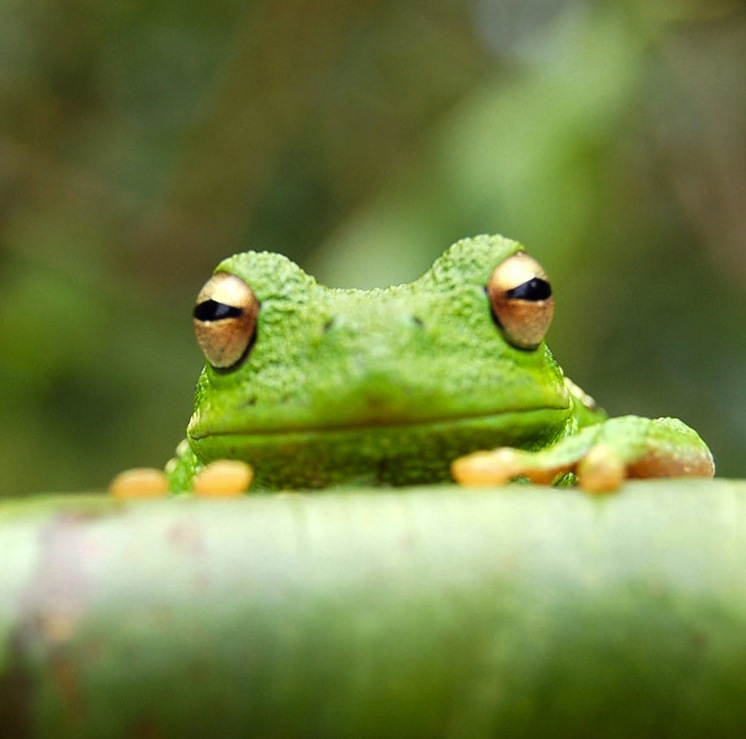
\includegraphics[width=\hsize]{frog}
\caption{A half-columnwidth image using wrapfigure, to be used sparingly. Note that using a wrapfigure before a sectional heading, near other floats or page boundaries is not recommended, as it may cause interesting layout issues. Use the optional argument to wrapfigure to control how many lines of text should be set half-width alongside it.}
\label{fig:halfwidth}
\end{wrapfigure}

Some filler text to sit alongside the half-width figure. \lipsum[1-2]

\begin{figure}
\begin{fullwidth}
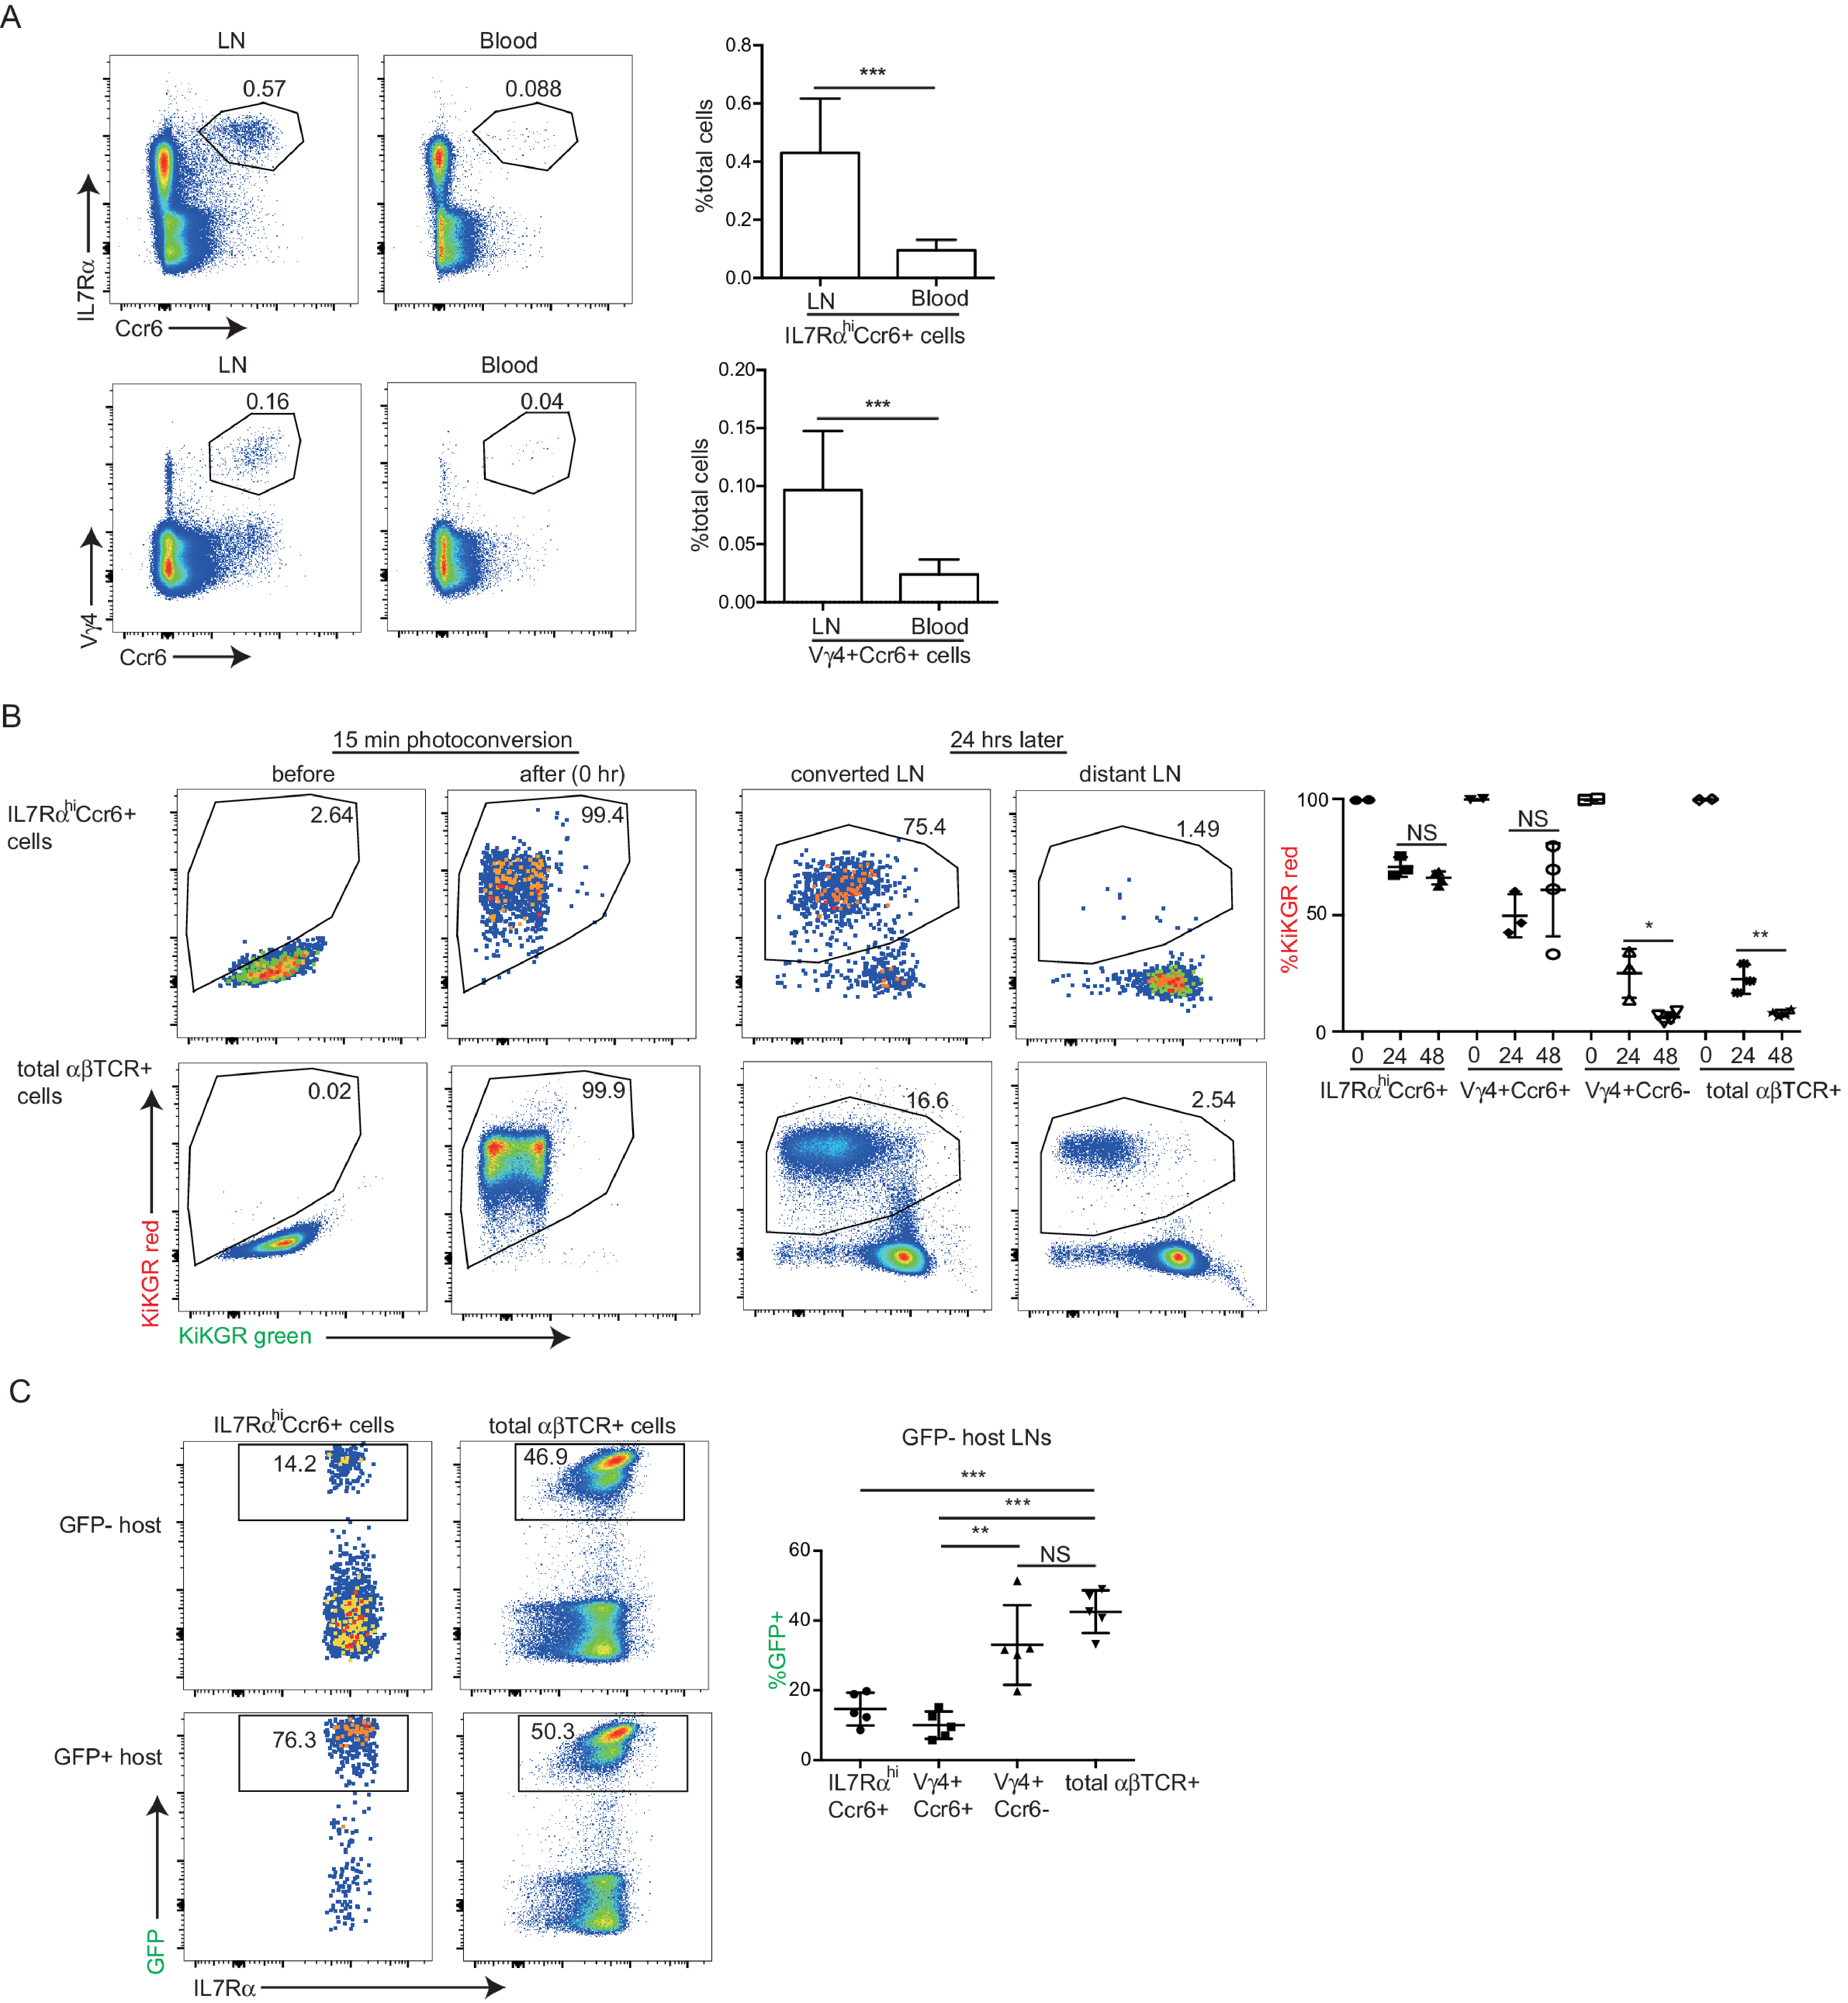
\includegraphics[width=0.95\linewidth]{elife-18156-fig2}
\caption{A very wide figure that takes up the entire page, including the gutter space.}
\label{fig:fullwidth}
\figsupp{There is no limit on the number of Figure Supplements for any one primary figure. Each figure supplement should be clearly labelled, Figure 1--Figure Supplement 1, Figure 1--Figure Supplement 2, Figure 2--Figure Supplement 1 and so on, and have a short title (and optional legend). Figure Supplements should be referred to in the legend of the associated primary figure, and should also be listed at the end of the article text file.}{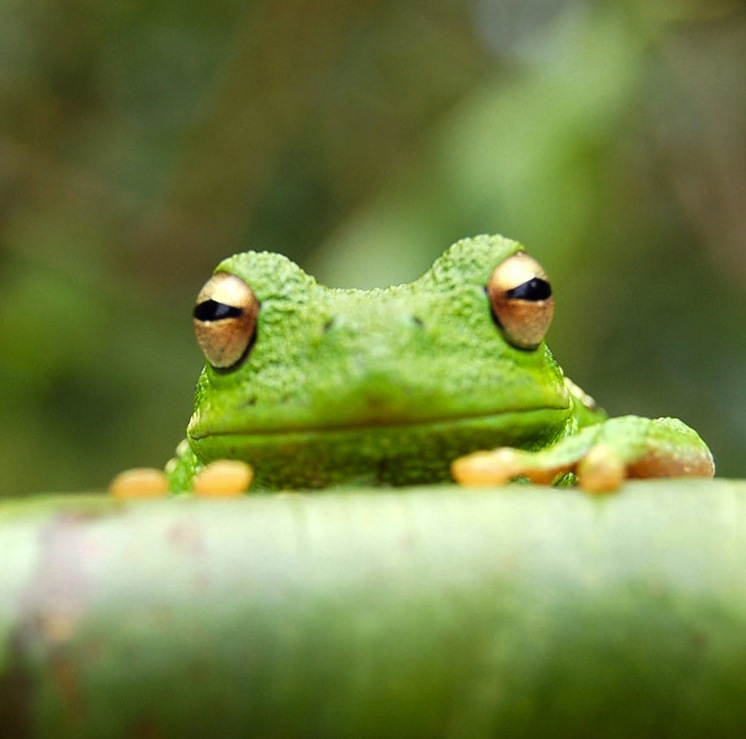
\includegraphics[width=5cm]{frog}}
\end{fullwidth}
\end{figure}

\subsection{Citations}

LaTeX formats citations and references automatically using the bibliography records in your .bib file, which you can edit via the project menu. Use the \verb|\cite| command for an inline citation, like \cite{Aivazian917}, and the \verb|\citep| command for a citation in parentheses \citep{Aivazian917}. The LaTeX template uses a slightly-modified Vancouver bibliography style. If your manuscript is accepted, the eLife production team will re-format the references into the final published form. \emph{It is not necessary to attempt to format the reference list yourself to mirror the final published form.} Please also remember to \textbf{delete the line} \verb|\nocite{*}| in the template just before \verb|\bibliography{...}|; otherwise \emph{all} entries from your .bib file will be listed! 

\begin{featurebox}
\caption{This is an example feature box}
\label{box:simple}
This is a feature box. It floats!
\medskip

\includegraphics[width=5cm]{example-image}
\featurefig{`Figure' and `table' captions in feature boxes should be entered with \texttt{\textbackslash featurefig} and \texttt{\textbackslash featuretable}. They're not really floats.}

\lipsum[1]
\end{featurebox}

\subsection{Mathematics}

\LaTeX{} is great at typesetting mathematics $abc$. Let $X_1, X_2, \ldots, X_n$ be a sequence of independent and identically distributed random variables with $\text{E}[X_i] = \mu$ and $\text{Var}[X_i] = \sigma^2 < \infty$, and let
\begin{equation}
\label{eq:CLT}
S_n = \frac{X_1 + X_2 + \cdots + X_n}{n}
      = \frac{1}{n}\sum_{i}^{n} X_i
\end{equation}
denote their mean. Then as $n$ approaches infinity, the random variables $\sqrt{n}(S_n - \mu)$ converge in distribution to a normal $\mathcal{N}(0, \sigma^2)$.

\lipsum[3] 

\begin{figure}
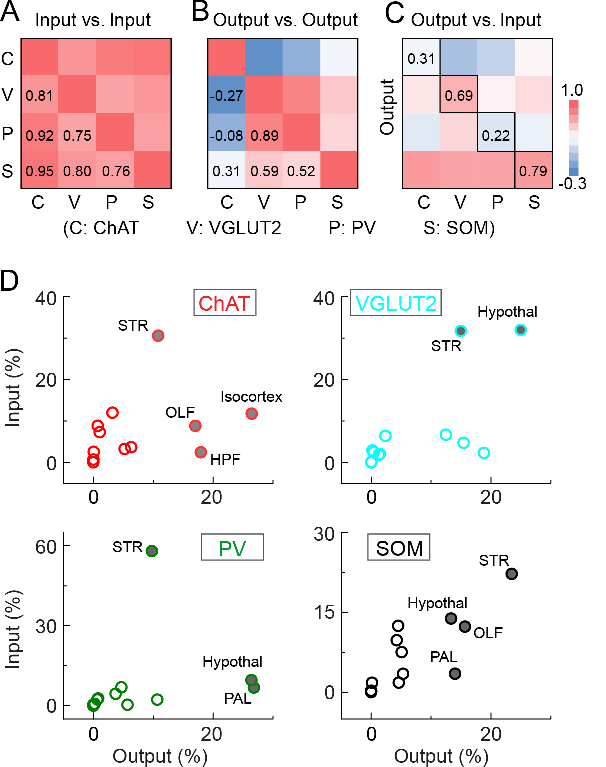
\includegraphics[width=\linewidth]{elife-13214-fig7}
\caption{A text-width example.}
\label{fig:view}
%% If the optional argument in the square brackets is "none", then the caption *will not appear in the main figure at all* and only the full caption will appear under the supplementary figure at the end of the manuscript.
\figsupp[Shorter caption for main text.]{This is a supplementary figure's full caption, which will be used at the end of the manuscript.}{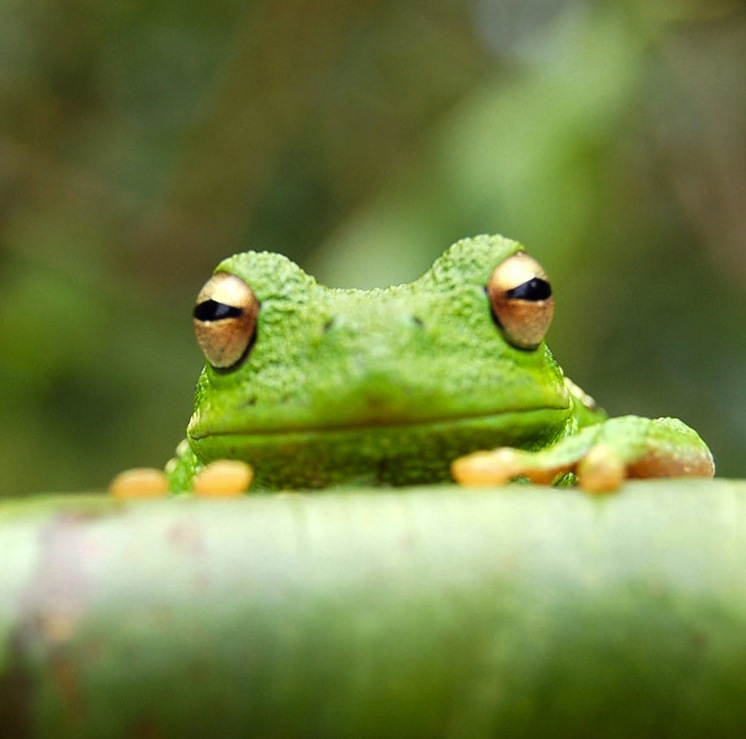
\includegraphics[width=6cm]{frog}}\label{figsupp:sf1}
\figsupp{This is another supplementary figure.}{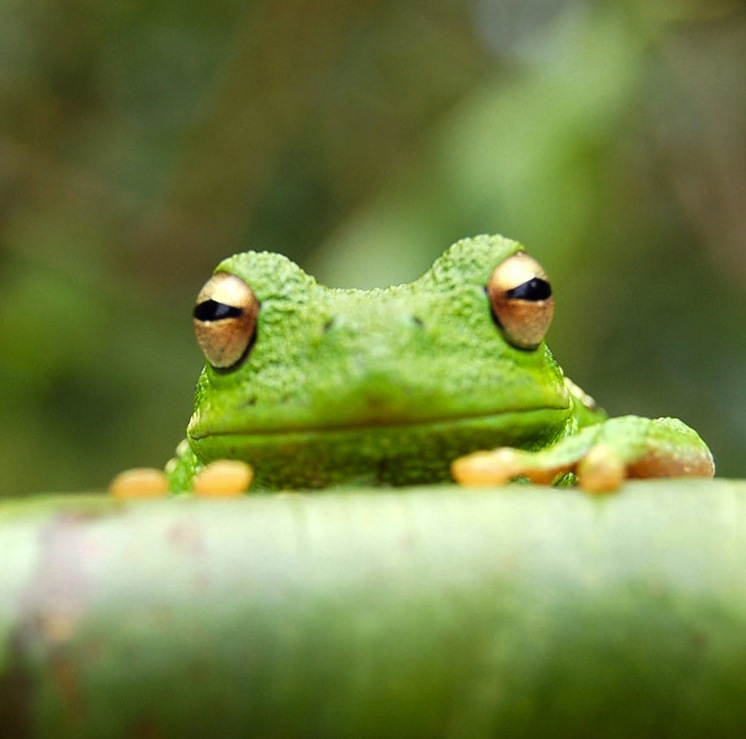
\includegraphics[width=6cm]{frog}}
\videosupp{This is a description of a video supplement.}\label{videosupp:sv1}
\figdata{This is a description of a data source.}\label{figdata:first}
\figdata{This is another description of a data source.}\label{figdata:second}
\end{figure}

\subsection{Other Chemistry Niceties}

You can use commands from the \texttt{mhchem} and \texttt{siunitx} packages. For example: \ce{C32H64NO7S}; \SI{5}{\micro\metre}; \SI{30}{\degreeCelsius}; \SI{5e-17}{\Molar}

\subsection{Lists}

You can make lists with automatic numbering \dots

\begin{enumerate}
\item Like this,
\item and like this.
\end{enumerate}
\dots or bullet points \dots
\begin{itemize} 
\item Like this,
\item and like this.
\end{itemize}
\dots or with words and descriptions \dots
\begin{description}
\item[Word] Definition
\item[Concept] Explanation
\item[Idea] Text
\end{description}

Some filler text, because empty templates look really poorly. \lipsum[1]


\section{Acknowledgments}

Additional information can be given in the template, such as to not include funder information in the acknowledgments section.

%\nocite{*} % This command displays all refs in the bib file. PLEASE DELETE IT BEFORE YOU SUBMIT YOUR MANUSCRIPT!
\bibliography{refs_Main_Report}

%%%%%%%%%%%%%%%%%%%%%%%%%%%%%%%%%%%%%%%%%%%%%%%%%%%%%%%%%%%%
%%% APPENDICES
%%%%%%%%%%%%%%%%%%%%%%%%%%%%%%%%%%%%%%%%%%%%%%%%%%%%%%%%%%%%

\appendix
\begin{appendixbox}
\label{first:app}
\section{Firstly}
\lipsum[1]

%% Sadly, we can't use floats in the appendix boxes. So they don't "float", but use \captionof{figure}{...} and \captionof{table}{...} to get them properly caption.
\begin{center}
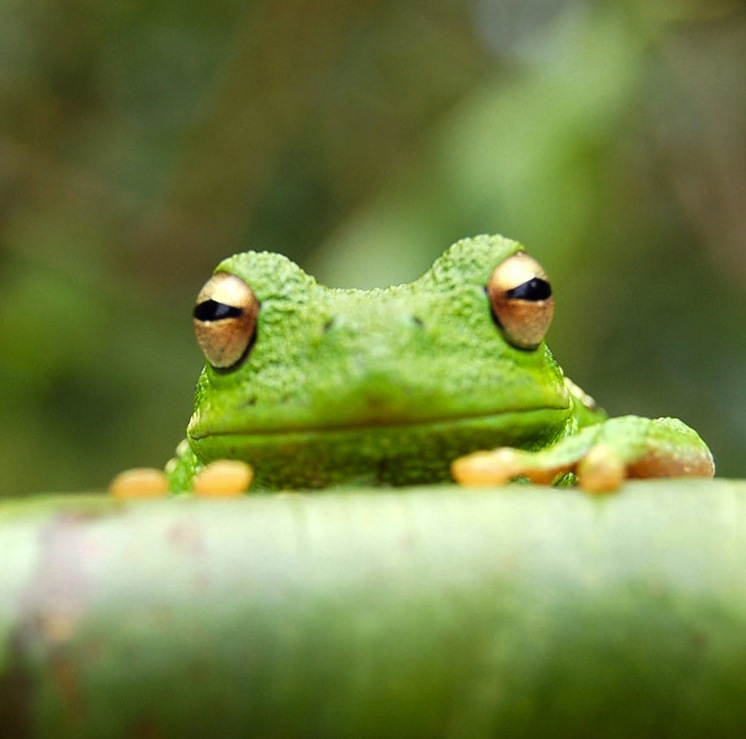
\includegraphics[width=\linewidth,height=7cm]{frog}
\captionof{figure}{This is a figure in the appendix}
\end{center}

\section{Secondly}

\lipsum[5-8]

\begin{center}
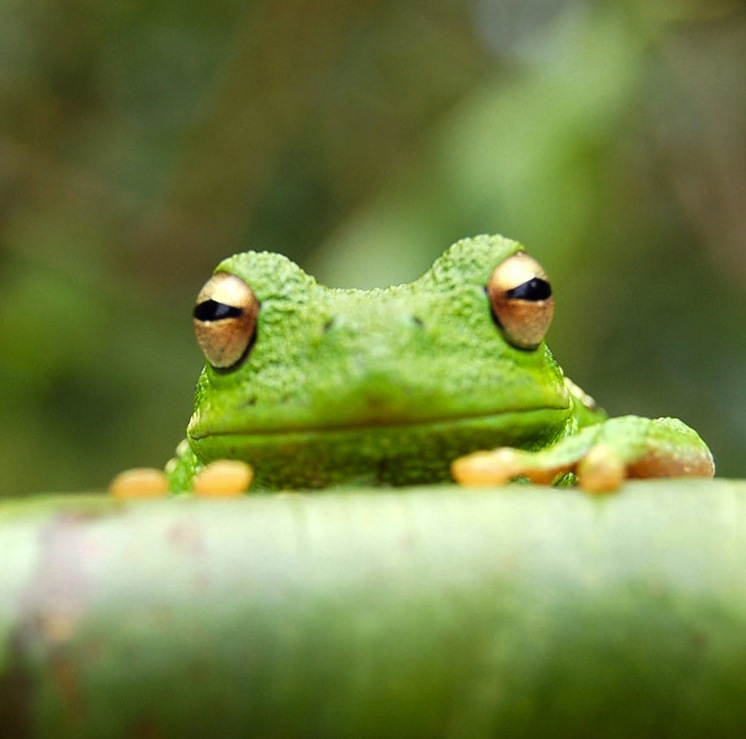
\includegraphics[width=\linewidth,height=7cm]{frog}
\captionof{figure}{This is a figure in the appendix}
\end{center}

\end{appendixbox}

\begin{appendixbox}
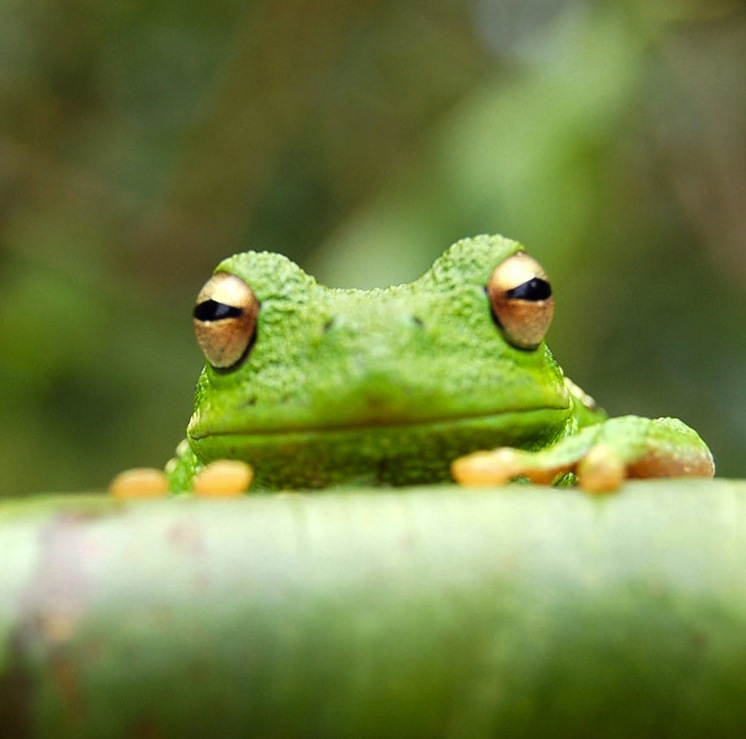
\includegraphics[width=\linewidth,height=7cm]{frog}
\captionof{figure}{This is a figure in the appendix}
\end{appendixbox}
\end{document}
